\documentclass[a4paper,12pt]{article}
\usepackage[finnish]{babel}
\usepackage[utf8]{inputenc}
\usepackage[pdftex]{graphicx}
\pagestyle{plain}
\begin{document}
\begin{titlepage}
\begin{center}
\textsc{\large Ohjelmoinnin harjoitustyö}\\[0.2cm] 
\textsc{\large Helsingin yliopisto, Tietojenkäsittelytieteen
laitos}\\[0.2cm]

\vspace{1cm}

\textsc{\LARGE WireworldEvolver määrittelydokumentti}

\vspace{2cm}

Jani Rahkola
jani.rahkola@cs.helsinki.fi

Ohjaaja: Jesse Lankila


\vfill
{\large \today}

\end{center}
\end{titlepage}

\section{Yleiskuvaus}
\paragraph{}
Soluautomaatti on diskreetti malli, joka koostuu ruudukosta soluja,
joilla on määrätty määrä tiloja joista yksi valiitsee kunakin hetkenä.
Solulla on naapurusto, joka koostuu soluautomaatin sääntöjen määräämistä
soluista. Solujen tilat muuttuvat sääntöjen perusteella, usein riipuen
solun naapurustoon kuuluvien solujen tiloista. Soluautomaatin tila
etenee askeleittain, ja jokaisella askeleella kaikkien solujen tila
arvioidaan, ja se muuttuu jos soluautomaatin säännöt niin määräävät.
\paragraph{}
Wireworld on Brian Silvermanin vuonna 1987 luoma soluautomaatti. Se
soveltuu erityisen hyvin loogisten piirien kuvaamiseen ja se on Turing
täydellinen. Wireworldissä solu voi olla yhdessä neljästä tilasta:
tyhjä (empty), johdin (conductor), elektronin pää (electron head) tai
elektronin häntä (electron tail). Solut ovat nelikulmioita taulukossa,
ja solun naapuruston muodostavat sitä ympäröivät 8 solua. Wireworld
solutaulukoita kutsutaan usein myös piireiksi, viittauksena loogisiin
piireihin, joita Wireworld soluautomaatilla usein mallinnetaan.
\paragraph{}
WireworldEvolver visualisoi ja simuloi Wireworld soluautomaatteja. Se
tarjoaa värikoodatun kuvauksen tekstitiedostona syötetystä
Wireworldpiiristä, ja mahdollistaa sen tilan kehittämisen askel kerrallaan tai
jatkuvasti.

\section{Rajoitukset}
Ohjelma sopii paremmin pienten soluautomaattien, kuten
loogisten piirien simuloimiseen, sillä piirin koko on rajoitettu
leveysuunnassa 70 soluun. Tämä siksi, että tekstitiedosto olisi
luettavissa useimmilla terminaaleilla ja tekstieditoreilla. Lisäksi
graafisen esityksen viemä tila ei pääse näin kasvamaan liian suureksi.

\section{Käsiteltävä data}
\paragraph{}
Wireworldpiiri syötetään ohjelmalle tekstitiedostona, jossa jokaista
solua kuvaa sen tilaa vastaava kokonaisluku 0-3. 0 vastaa tyhjää solua,
1 elektronin päätä, 2 elektronin häntää ja 3 johdinta. Kaikki muut
merkit sivuutetaan. Visualisoitavan taulukon rivien määräksi tulee
tiedoston rivien määrä, ja sarakkeiden määräksi ensimmäisen rivin
merkitsevien merkkien määrä.
\paragraph{}
Käyttöliittymän kautta käyttäjältä saadaan tekstimuotoisena avattavan
tiedoston polku, ja nappien ja liukusäätimen kautta tapahtumia, joilla
ohjelman suoritusta ohjataan.

\section{Datan kulku}
\paragraph{}
Käyttäjältä saadaan tiedostopolku, joko tekstisyötteenä tai
tiedostovalitsimen kautta. Polun tiedosto avataan, jos mahdollista, ja
tiedoston sisältö kopioidaan sisäiseen tietorakenteeseen. Tiedosto
suljetaan, jotta sitä voidaan muokata ohjelman ajon aikana.
\paragraph{}
Käyttäjälle esitettävät virheilmoitukset, kuten tiedoston avaukseen
liittyvät virheet, näkyvät tekstinä käyttöliittymän pääikkunassa.
\paragraph{}
Wireworldpiirin visualisaatio on erivärisistä soluista koostuva
taulukko, jossa väri kuvaa solun tilaa.
\newpage
\section{Toiminnot ja ohjelman käyttö}
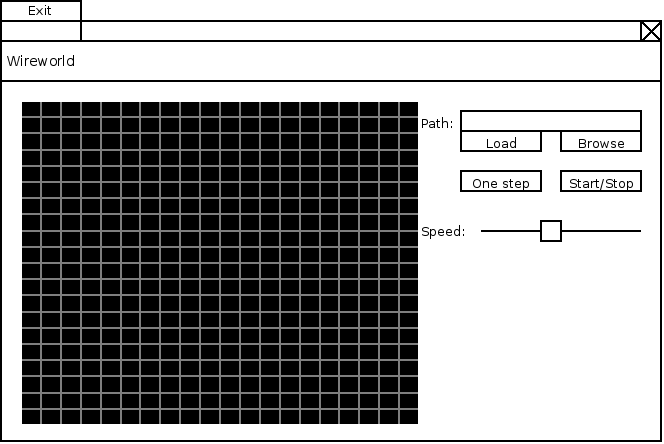
\includegraphics[width=5in]{KayttoliittymaMaarittely.png}
\begin{description}
\item[Ohjelman sulkeminen:] Joko ikkunointimanagerin tarjoaman 'sulje ikkuna'
-napin kautta, tai Wireworld valikosta löytyvällä Exit valinnalla.
\end{description}

\begin{description}
\item[Wireworldpiirin lataaminen:] Syötetään tiedoston polku Path: -kenttään
ja painetaan Load -nappia. Piiri visualisoituu käyttöliittymän
taulukkoon. Jos tiedostoa ei löydy, ilmoitetaan tämä tekstinä Path:
-kentän alla.
Vaihtoehtoisesti käyttäjä painaa Browse -nappia ja etsii haluamansa
tiedoston tiedostovalitsimen avulla.
\end{description}

\begin{description}
\item[Wireworldpiirin uudelleenlataaminen:] Piirin sisältävää tiedostoa
voidaan muokata ohjelman ollessa käynnissä, ja se voidaan ladata
uudelleen kuten ensimmäiselläkin kerralla.
\end{description}

\begin{description}
\item[Piirin tilan edistäminen yhdellä askel kerralaan:] Painamalla One step
-nappia piirin tila edistyy yhden askeleen (generation).
\end{description}

\begin{description}
\item[Piirin tilan jatkuvan edistämisen käynnistäminen:] Start/Stop -nappi käynnistää
piirin jatkuvan edistämisen Speed -liukusäätimen määräämällä nopeudella.
\end{description}

\begin{description}
\item[Piirin tilan jatkuvan edistämisen pysäyttäminen:] Start/Stop -nappi
pysäyttää piirin jatkuvan edistämisen ja pysäyttämishetken tila jää
visualisoiduksi.
\end{description}

\begin{description}
\item[Piirin tilan jatkuvan edistämisen nopeuden säätö:] Speed -liukusäätimellä
asetetaan edistämisen nopeus. Absoluuttisia arvoja ei esitetä
käyttäjälle.
\end{description}

\begin{description}
\item[Piirin tilan alustaminen:] Piirin saattaminen tiedostossa
määritettyyn tilaan tapahtuu lataamalla piiri uudestaan.
\end{description}

\end{document}                                               
